How to world

\subsubsection{Sky}
The sky is achieved using a high-resolution texture of a sky mapped to a skybox. The mathematical location of the sun is placed as close as possible to the sun appearing in this texture. This gives shadows and shading a natural feel. The texture has been manually modified at the horizon to fade towards a shadowish gray color. The color is the same as the one objects are distance-fogged with. This makes the sky melt into the ocean in a very nice way. 

\subsubsection{Ocean}
// TODO  Tiger \\
Normal-mapped square

\subsubsection{Terrain}
The terrain is generated by sampling a noise function and translating its value into a height for the current vertex. The noise in this case originates from a Simplex function. However, to get a realistically looking terrain one it is not sufficient to sample this function only once for every vertex.

Fractional Brownian Motion is calculated by sampling the Simplex function at different frequencies and calculating a weighted sum over the samples \cite{FracBrownMotion}. The result is a nice looking height map. 

\begin{figure}[H]

\begin{subfigure}{.5\textwidth}
  \centering
  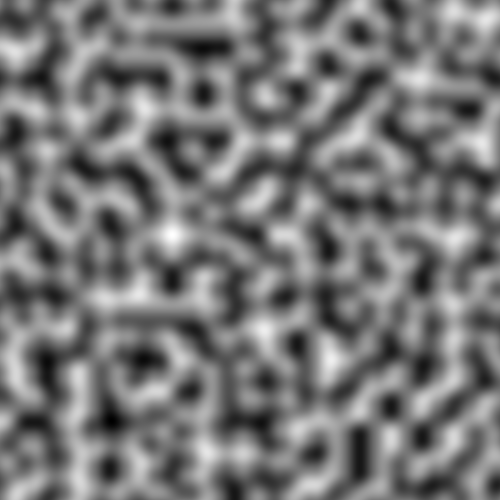
\includegraphics[width=0.9\linewidth]{images/Simplex.png}
  \caption{Height map generated from single-octave simplex noise}
  \label{fig:sub1}
\end{subfigure}%
\begin{subfigure}{.5\textwidth}
  \centering
  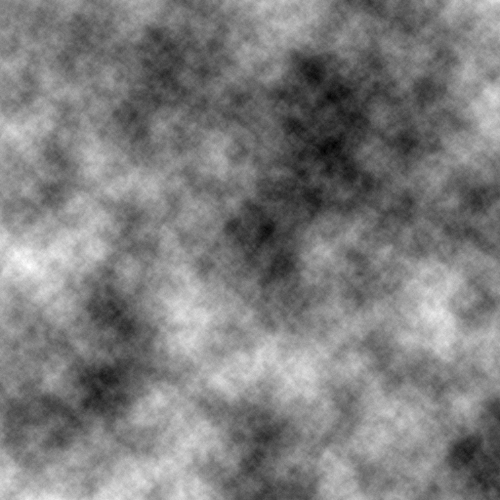
\includegraphics[width=0.9\linewidth]{images/FracBrownMotion.png}
  \caption{Height map generated with Fractional Brownian Motion}
  \label{fig:sub2}
\end{subfigure}
\caption[Noise comparison]{\textit{Comparison of noise functions}}
\label{fig:R_kitchen_example}
\end{figure}

\subsubsection{Content}
// TODO - Häger \\
Trees and rocks 





